%%This is a very basic article template.
%%There is just one section and two subsections.
\documentclass{article}
\usepackage{graphicx}

\setlength{\parskip}{1em}

\begin{document}


\section{Editing Meshes}

This document is designed to outline the basic user controls of the Mesh Editor plugin in ICE.

\subsection{Getting Started}

Once ICE is installed on your system, there are no addional dependencies or
preparation required to use the Mesh Editor.

\subsubsection{Opening a Mesh Editor}

To open a Mesh Editor in ICE, you have four options:
 

\begin{center}
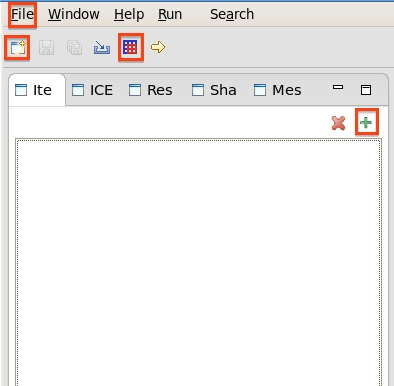
\includegraphics[height=5cm]{images/CreateNewMeshOptions.jpg}
\end{center}

The UI elements which can be used to open a Mesh Editor are
highlighted. Instruction for how to use each one, from top to bottom, left to
right, are given below.

 
1) Click the File menu, then New, then Create Item Wizard.

 
2) Click the New Item Button and select Create Item Wizard.


3) Click the Mesh Editor button.


4) In the ICE Perspective, click the Create an Item button, select Mesh Editor,
and click OK.

\section{Working With the Mesh Editor}

The mesh editor will initially open to an empty grid, as shown below. There is
currently no way to import pre-existing meshes from another source directly
into the Mesh Editor.

\begin{center}
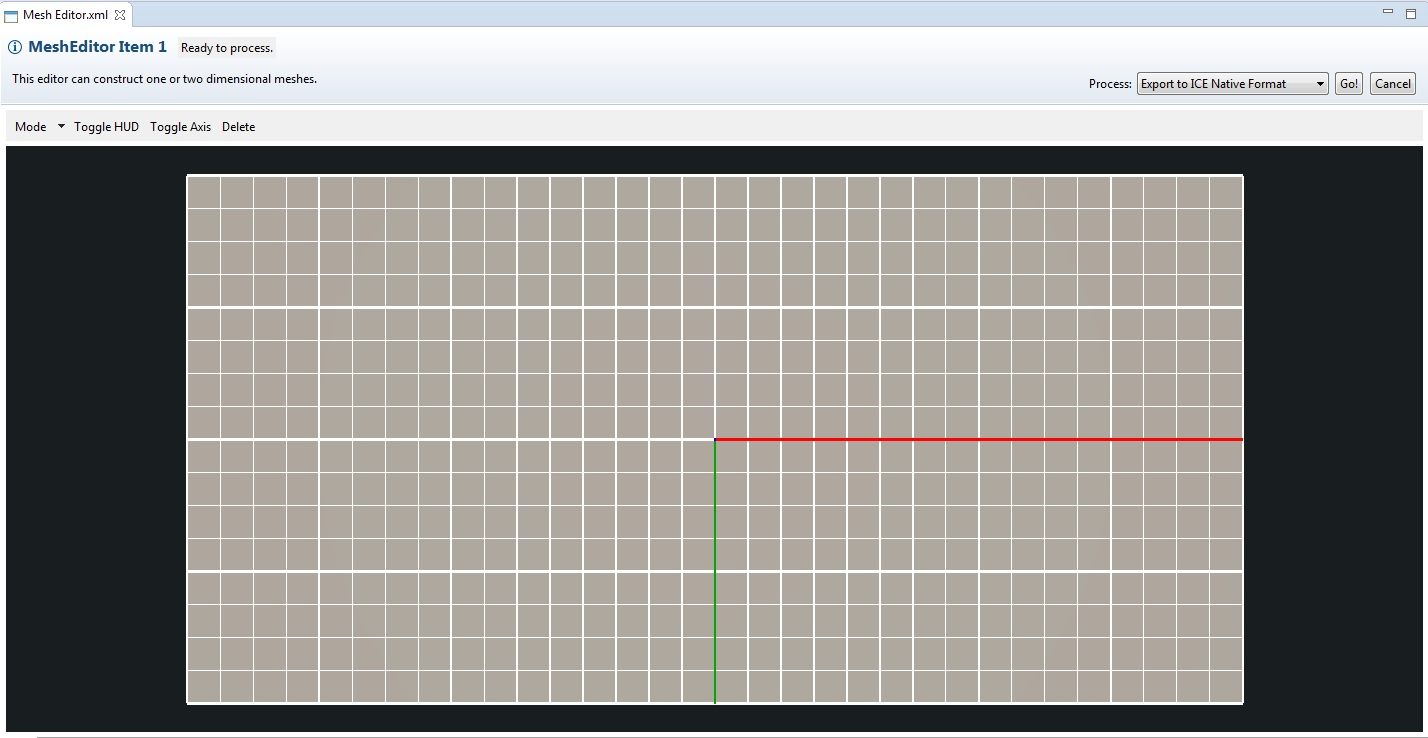
\includegraphics[width=12cm]{images/EmptyMeshEditor.jpg}
\end{center}

\subsection{Navigation}

Meshes are constructed on the background grid. Gridlines are spaced one unit
apart from each other. The origin is the initial center of the screen, with the
x axis in red and the y axis in green coming out from it in the positive x and y
directions, respectively. 

\subsubsection{Camera Controls}

The camera is controlled with keyboard and mouse commands. The W, A, S, and D
keys are used to move the camera around the editor's area, while scrolling the
mouse wheel is used to zoom the camera in and out. 

If the controls are not working, ensure that the Mesh Editor has focus by
clicking inside of it.

\begin{center}
    \begin{tabular}{| l | l |}
    \hline
    \multicolumn{2}{|c|}{\textbf{Camera Controls}} \\
  	\hline
    \textbf{Action} & \textbf{Key(s)} \\ \hline
    Scroll Up & W \\ \hline
    Scroll Down & S \\ \hline
    Scroll Left & A \\ \hline
    Scroll Right & D \\ \hline
    Zoom In & Scroll mouse wheel up \\ \hline
    Zoom out & Scroll mouse wheel down \\
    \hline
    \end{tabular}
\end{center}

\subsection{Adding Elements}

2D meshes are constructed in the editor by specifying one quadtrilatiral at a
time. To add a new polygon, the Mesh Editor must be in Add Elements Mode. This
is the editor's default setting, and it can later be reset by clicking the Mode
button in the top left corner. 

\begin{center}
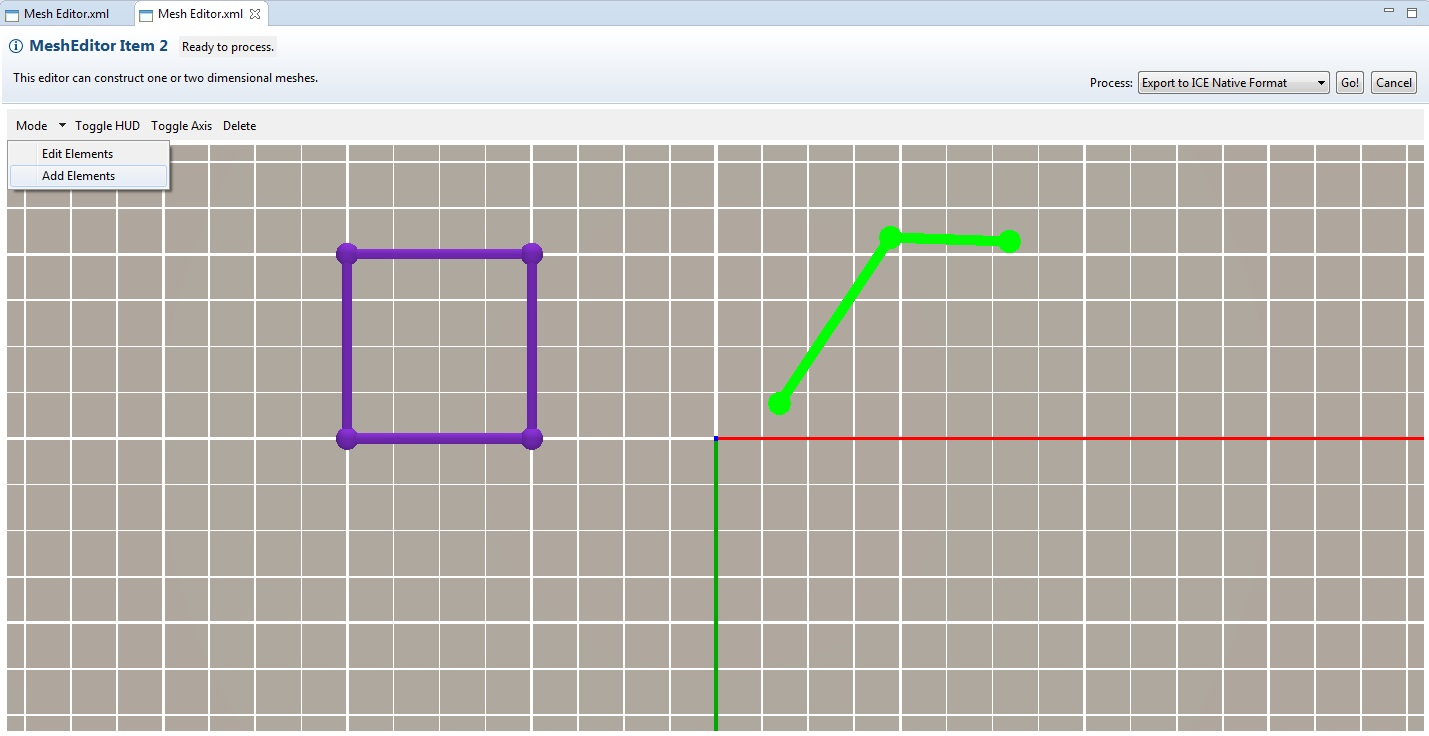
\includegraphics[width=12cm]{images/MeshEditorAddMode}
\end{center}

\subsubsection{Placing Vertices}

In Add Elements Mode, clicking anywhere on the grid will place a new vertex at
that location. These new, temporary vertices and the edges between them will be
colored in green, to show that the polygon in still under construction.

Alternatively, you may select a vertex not already in the new polygon. This
allows you to reuse vertices and/or edges already present in the mesh to form
part of your new polygon.

\begin{figure}
\begin{center}
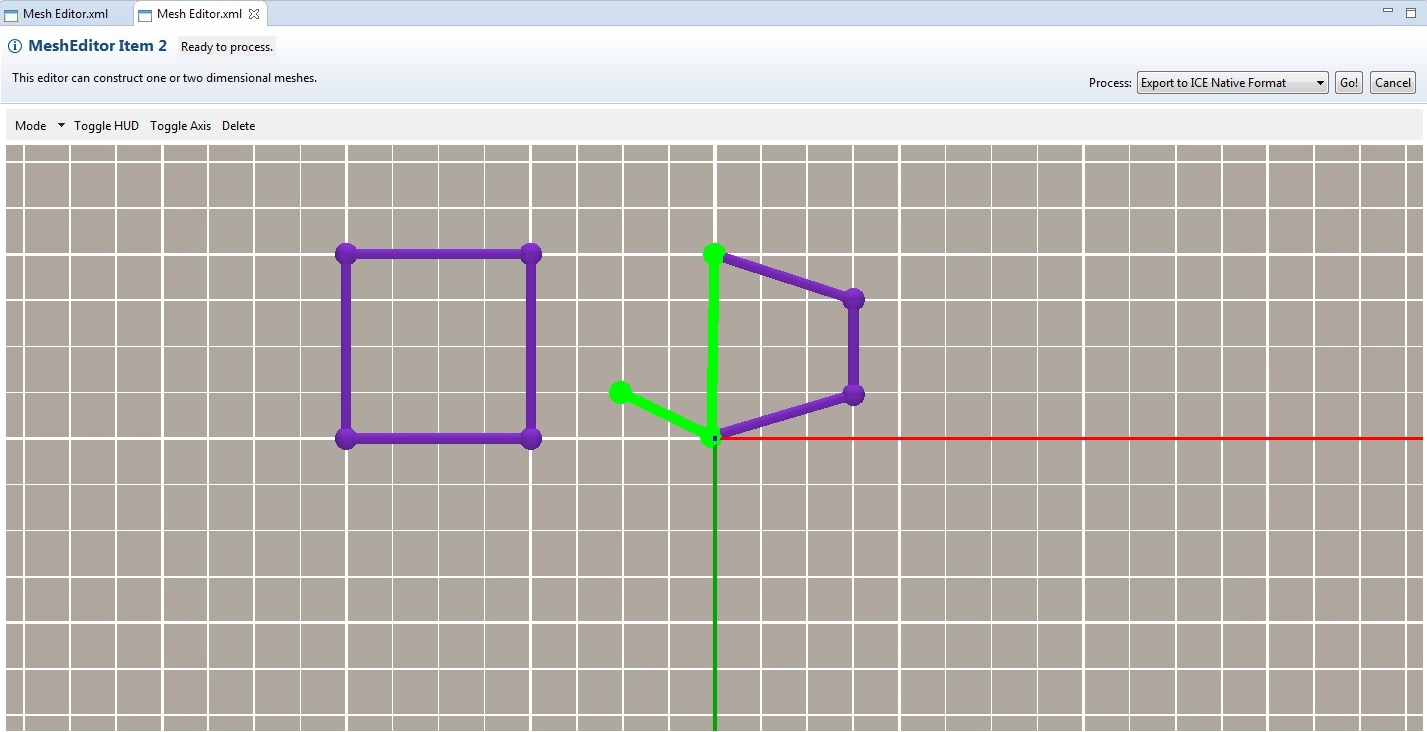
\includegraphics[width=12cm]{images/MeshEditorReuseEdge}
\caption{One of the edges from the trapezoid is being combined with a new edge
in the creation of the current polygon.}
\end{center}
\end{figure}

Once the fourth vertex has been specified, the polygon will change to purple to
show that it has been completed. At any time before this, you can press the Esc
button to cancel the new polygon, removing it from the editor and allowing you
to start the process over. 

\subsection{Editing Elements}

To edit an already present element of the mesh, you must switch to Edit Elements
Mode. The Mode button in the upper left corner alows you to switch between
modes, as shown below.

\begin{center}
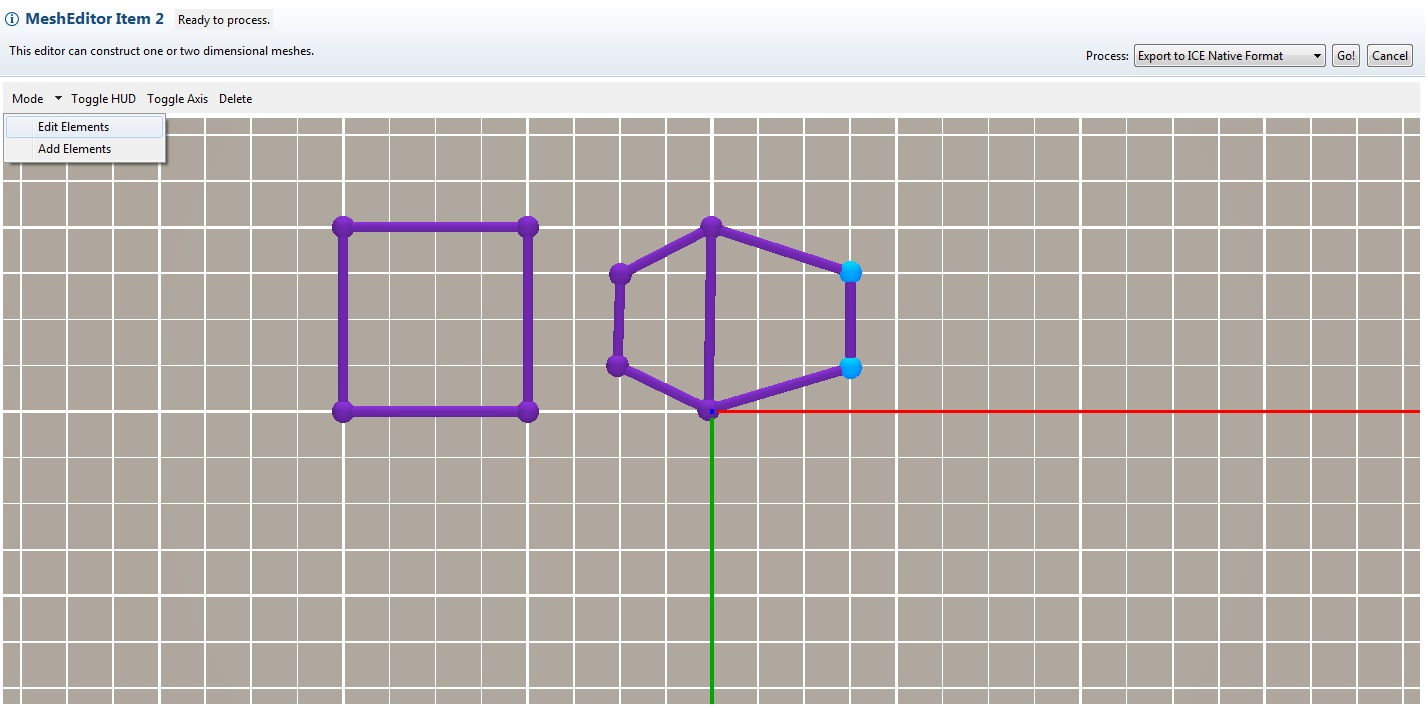
\includegraphics[width=12cm]{images/MeshEditorEditMode}
\end{center}

A vertex can be selected by either clicking it in the Mesh Editor, or by
selecting it from the tree in the ICE Perspective's Mesh Elements View. Holding
down shift while clicking will allow multiple vertices to be selected at once,
while holding down control during a click will toggle a vertex's state either
into or out of the selection. Selected elements are displayed in blue.
The current selection can be cleared by pressing the Esc button.

\begin{center}
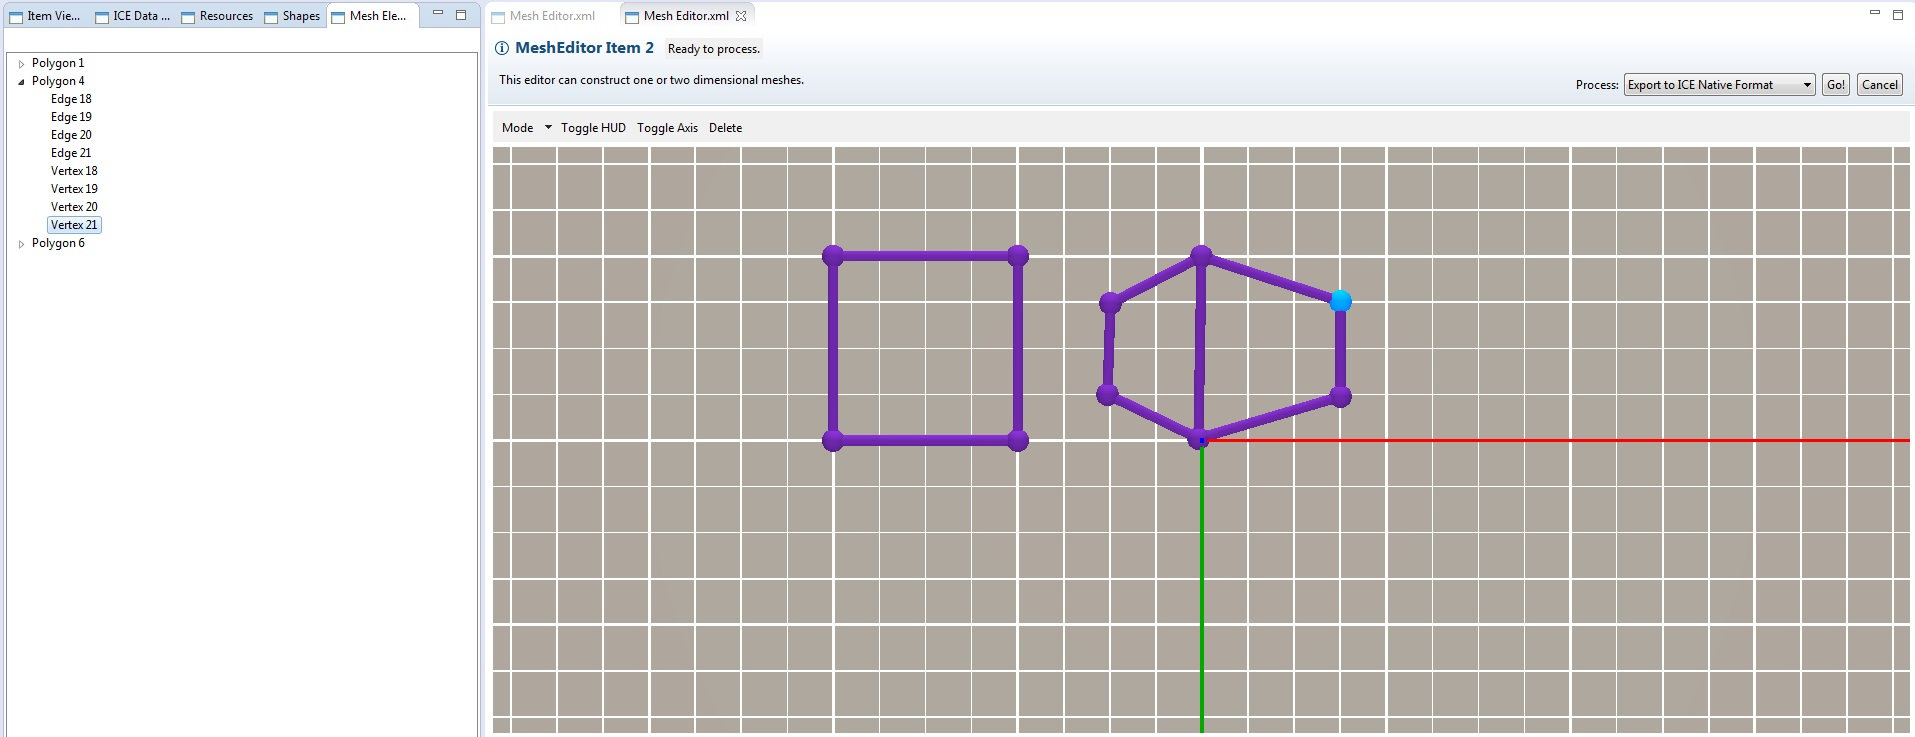
\includegraphics[width=12cm]{images/MeshEditorSelection}
\end{center}

Click on a selected vertex and drag it to change its location. The clicked
vertex will stay beneath your mouse cursor, while all other selected vertices
will be moved as well, keeping their relative position to the dragged vertex.
White circles are displayed to show each vertex's new location. Pressing Escape
during the drag will deselect the vertices and cancel the movement.

\begin{figure}
\begin{center}
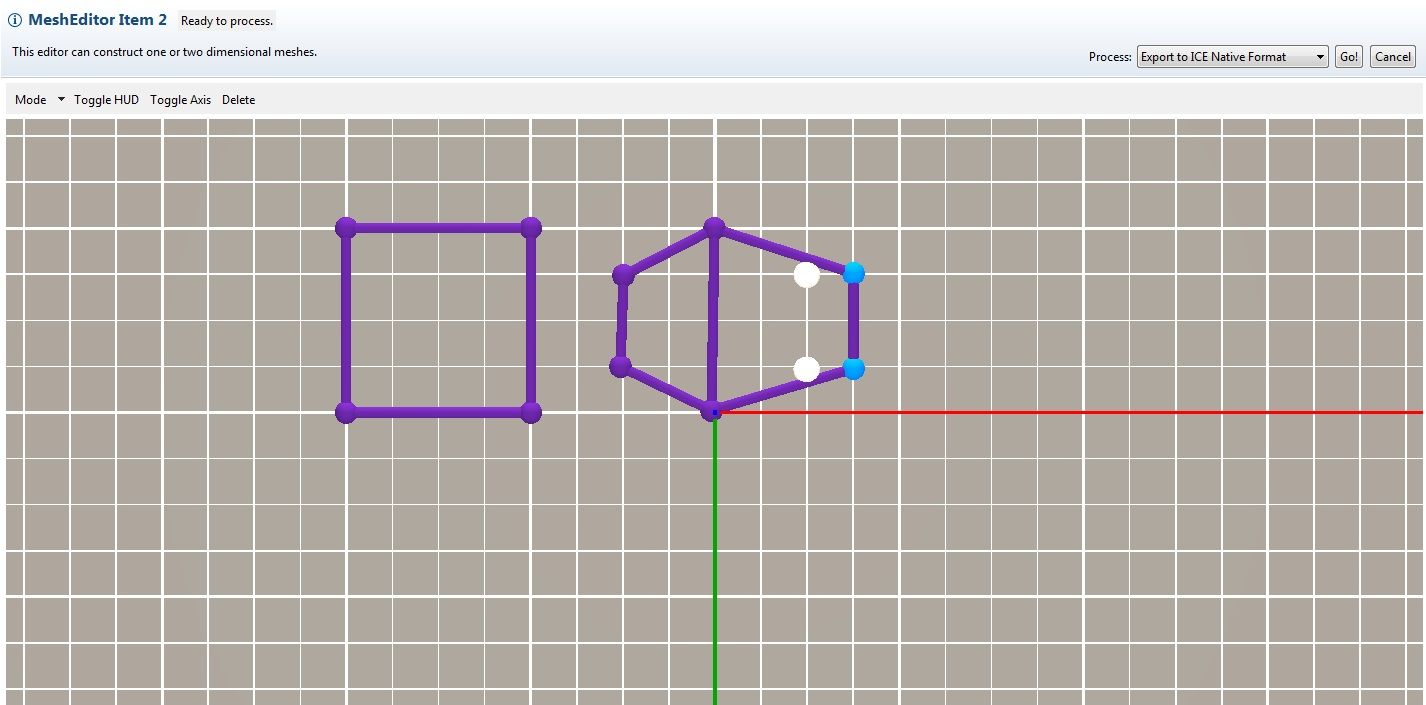
\includegraphics[width=12cm]{images/MeshEditorDragVertex}
\caption{Two vertices are selected. When the bottom vertex is moved left, the
top vertex is moved left by an equal amount.}
\end{center}
\end{figure}

\begin{center}
    \begin{tabular}{| l | l |}
    \hline
    \multicolumn{2}{|c|}{\textbf{Edit Mode Controls}} \\
  	\hline
    \textbf{Action} & \textbf{Key(s)} \\ \hline
    Select vertex & Left click \\ \hline
    Add to selection & Shift + left click \\ \hline
    Toggle (Add/Remove) Selection & Ctrl + left click \\ \hline
    Move selected vertices & Left click on vertex and drag mouse \\ \hline
    Clear selection/Cancel move & Escape \\ 
    \hline
    \end{tabular}
\end{center}

Alternatively, you can edit a vertex more precisely by setting its exact
coordinates. First, select it in the Mesh Elements view, then open the
Properties View. The vertex's x and y coordinates will be displayed in editable
text boxes.

\begin{center}
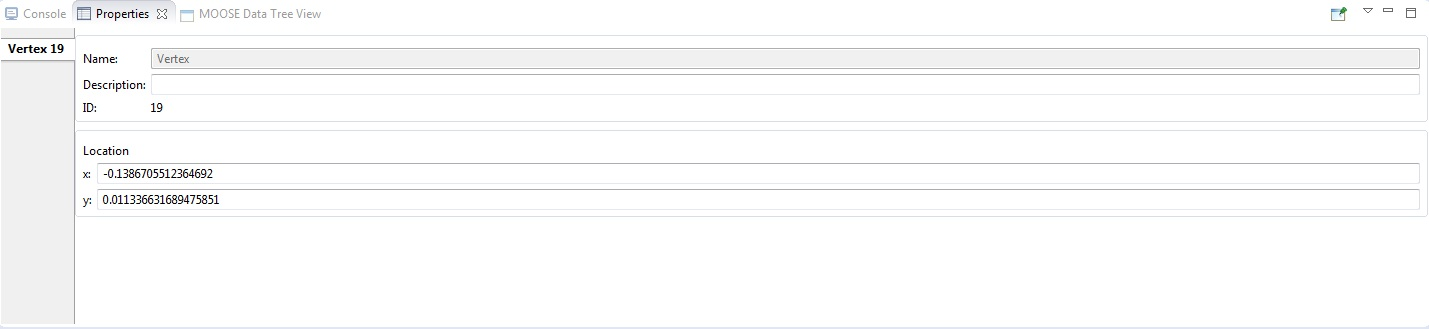
\includegraphics[width=12cm]{images/VertexPropertiesView}
\end{center}

Selecting a polygon in the same way, then opening the tab for one of its edges
in the Properties View, will display the edge's boundary conditions for that
polygon. These are editable, just like the vertices are.

\begin{center}
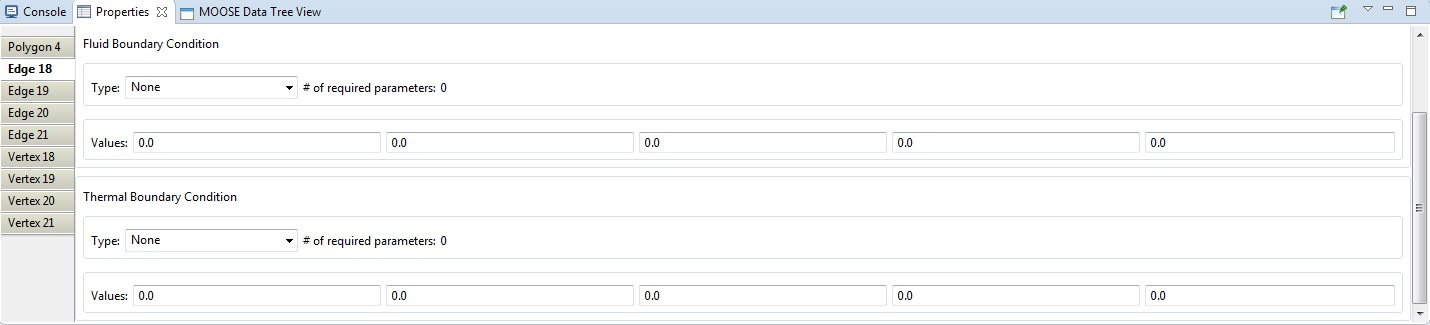
\includegraphics[width=12cm]{images/EdgeBoundaryConditions}
\end{center}

\subsection{Deleting Elements}

Polygons in the mesh can be deleted. All four vertices for the polygon must be
selected, then press the Delete button on the toolbar. Vertices and edges which
are still part of other, undeleted, polygons will remain, but all others will be
removed from the editor.

\subsection{Additional Controls}

The Toggle Axis button on the toolbar allows will add/remove the axes from the
editor. 

\begin{center}
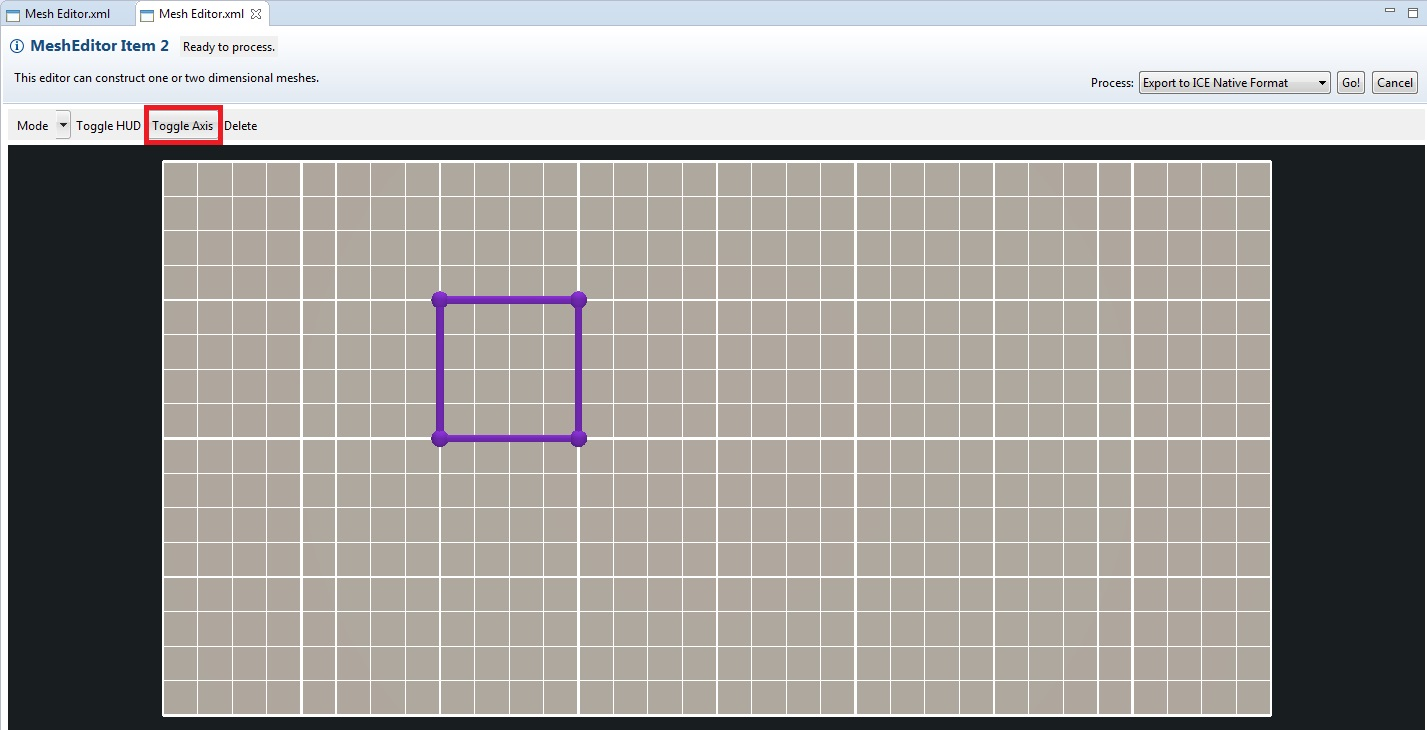
\includegraphics[width=12cm]{images/MeshEditorToggleAxis}
\end{center}

\end{document}
